\subsection{Test} \label{test}

Tale sezione ha lo scopo di spiegare il funzionamento, lo scopo e i risultati dei vari tipi di test proposti dal modello a V e che adottiamo.

\subsubsection{Modello a V} \label{sezionemodelloV}
Il modello a V descrive in modo sintetico il ciclo di vita della realizzazione del software, partendo dalla sua progettazione fino alla sua consegna al cliente escludendo la fase di manutenzione.

Lo scopo del modello a V è quello di mostrare quali tipi di test accompagnano ogni fase del ciclo e di come anche questi siano propedeutici l'uno dall'altro.

\begin{figure}[H]
	\centering
	%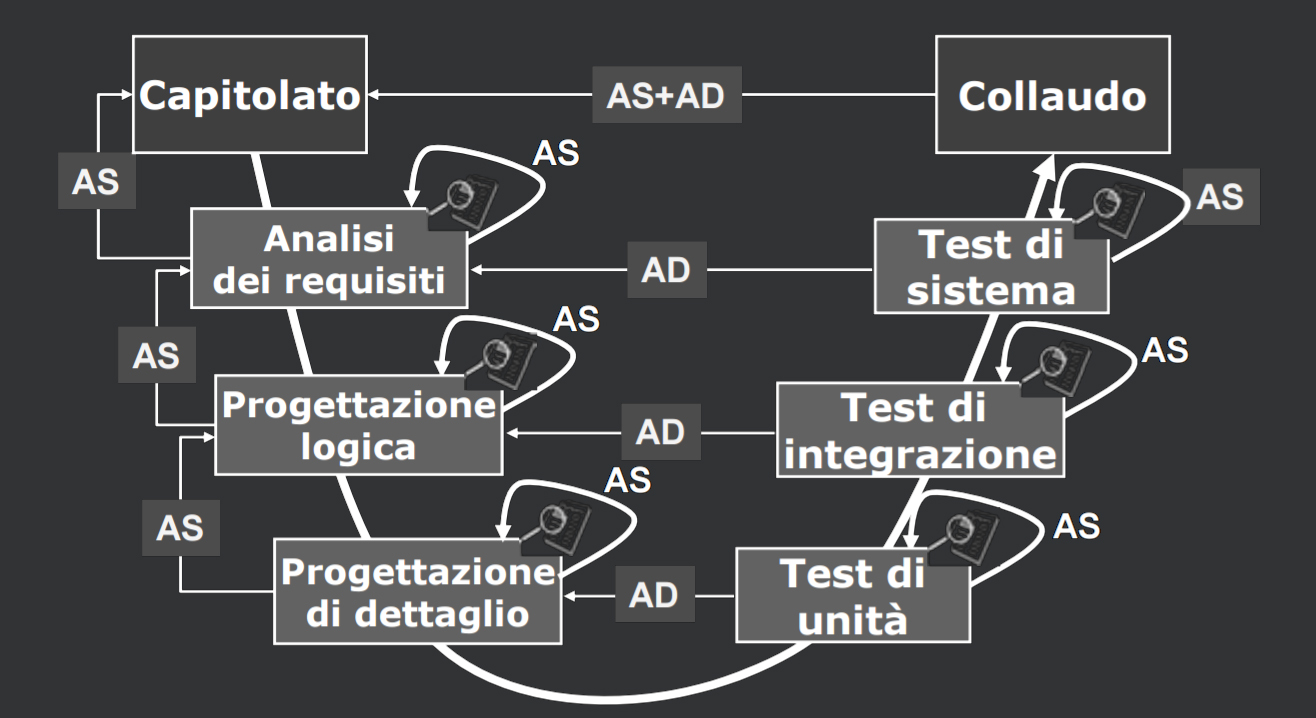
\includegraphics[width=0.8\textwidth]{img/modellov-sweki.jpg}
	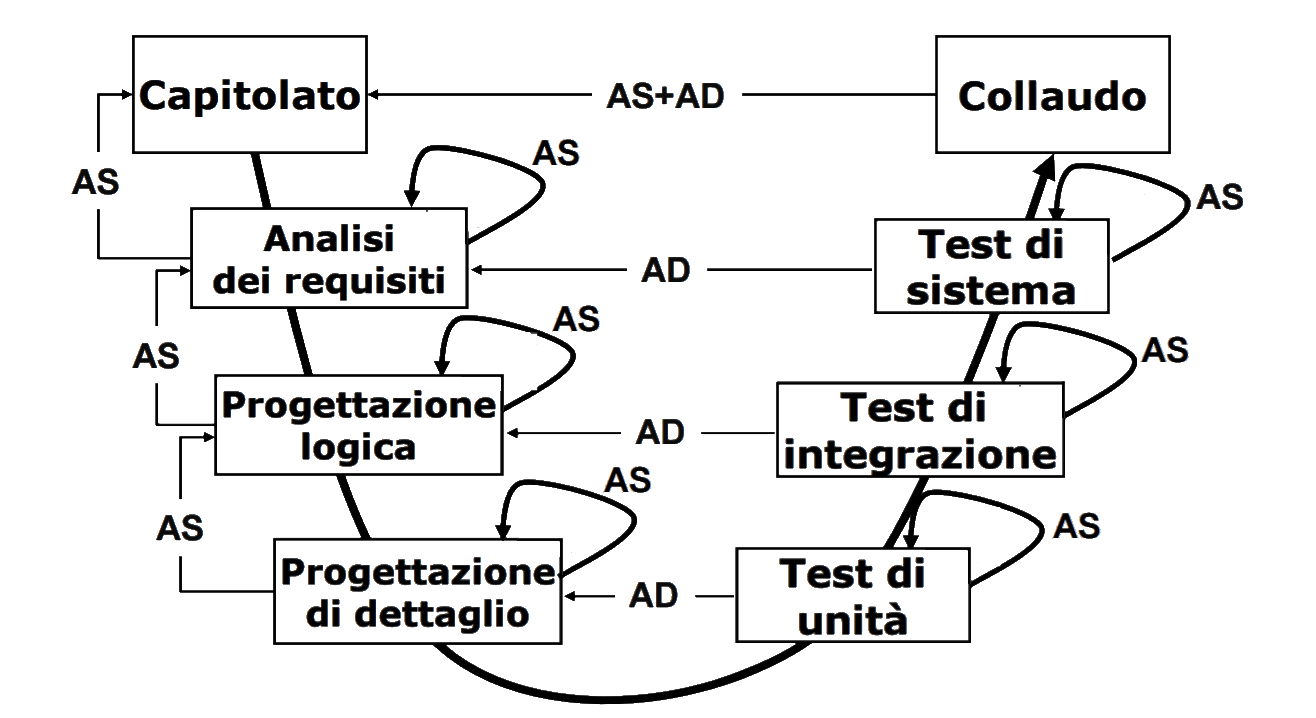
\includegraphics[width=0.8\textwidth]{img/modellov-sweki_inv.png}
	\caption[Modello a V]{Modello a V\protect\footnotemark}
	\label{img:vmodel}
\end{figure}

\footnotetext{Riferirsi alla voce ``6. Modello a V'' in  \S\ref{riferimenti informativi}}

\subsubsection{Classificazione e stuttura dei test} \label{classificazionetest}
Ogni test viene identificato univocamente dal seguente codice:

\begin{center}
	\texttt{T[Tipo][ID]}
\end{center}

\begin{itemize}
	\item \textbf{T}: si riferisce a ``Test''.
	\item \textbf{Tipo}: la tipologia a cui il test appartiene che, seguendo il modello a V\footnote{\url{https://en.wikipedia.org/wiki/V-Model_(software_development)}}, può essere:
	\begin{itemize}
		\item \textbf{V}: validazione. %è la stessa cosa di collaudo e di accettazione??
		\item \textbf{S}: sistema
		\item \textbf{I}: integrazione.
		\item \textbf{U}: unità.
		\end{itemize}
	%per la corrispondenza con i requisiti, non vanno bene le "tre cifre"
	\item \textbf{ID}: numero incrementale che rispetta una struttura gerarchica.
\end{itemize}

% COLORI
\newcommand{\TNI}{{\color{gray}\textbf{NI}}}
\newcommand{\TI}{{\color{blue}\textbf{I}}}
\newcommand{\TNS}{{\color{red}\textbf{NS}}}
\newcommand{\TS}{{\color{green}\textbf{S}}}

Le tabelle che raccolgono i test di una determinata tipologia presentano i campi:
\begin{itemize}
	\item \textbf{Codice}: comprendente il codice identificativo del test.
	\item \textbf{Test}: descrive cosa il test deve verificare.
	\item \textbf{Stato}: indica lo stato del test e può essere:
	\begin{itemize}
		\item \TNI: non implementato.
		\item \TI: implementato ma non ancora avviato.
		\item \TNS: avviato e fallito.
		\item \TS: avviato e superato.
	\end{itemize}
\end{itemize}

\subsubsection{Test di validazione} \label{testvalidazione}
È un tipo di test da determinare e sviluppare in parallelo con la comprensione del capitolato.
Come si può vedere dal modello a V (figura \ref{img:vmodel}), sono i primi tipi di test che vengono creati e saranno gli ultimi ad essere eseguiti prima della consegna del prodotto.

\newenvironment{VTtable}[1][1]{%
	\renewcommand*{\arraystretch}{#1}%
	\renewcommand\theadfont{\bfseries}%
	\oldtabularx%
}{\endoldtabularx}

\newcounter{tv}
\newcommand{\addtotv}{\stepcounter{tv}TV\thetv}

\newcounter{tableCounter}

\stepcounter{tableCounter}
\begin{table}[H]
	\begin{VTtable}[1.7]{\textwidth}{cXc}
		\rowcolor{\tablegray}
		\textbf{Codice} & \centering\textbf{Test} & \textbf{Stato} \\\toprule
		\addtotv & Verifica la segnalazione dell'apertura di una issue in Redmine:
		\begin{enumerate}
			\item Viene aperta una issue in Redmine.
			\item Redmine invia la segnalazione.
            \item Producer Redmine riceve la segnalazione da Redmine.
		\end{enumerate}
		& \TI \\\midrule

        \addtotv & Verifica la segnalazione della modifica di una issue in Redmine:
		\begin{enumerate}
			\item Viene modificata una issue in Redmine.
			\item Redmine invia la segnalazione.
            \item Producer Redmine riceve la segnalazione da Redmine.
		\end{enumerate}
		& \TI \\\midrule

        \addtotv & Verificata la segnalazione del commento di una issue in Redmine:
        \begin{enumerate}
            \item Viene commentata una issue in Redmine.
            \item Redmine invia la segnalazione.
            \item Il Producer Redmine riceve la segnalazione da Redmine.
        \end{enumerate}
        & \TI \\\midrule

        \addtotv & Verifica la segnalazione dell'apertura di una issue in GitLab:
		\begin{enumerate}
			\item Viene aperta una issue in GitLab.
			\item GitLab invia la segnalazione.
            \item Producer GitLab riceve la segnalazione da GitLab.
		\end{enumerate}
		& \TI \\
        \bottomrule
	\end{VTtable}
	\caption{Elenco dei test di validazione (\thetableCounter)}
\end{table}

\stepcounter{tableCounter}
\begin{table}[H]
	\begin{VTtable}[1.7]{\textwidth}{cXc}
		\rowcolor{\tablegray}
		\textbf{Codice} & \centering\textbf{Test} & \textbf{Stato} \\\toprule

        \addtotv & Verifica la segnalazione della modifica di una issue in GitLab:
        \begin{enumerate}
            \item Viene modificata una issue in GitLab.
            \item GitLab invia la segnalazione.
            \item Producer GitLab riceve la segnalazione da GitLab.
        \end{enumerate}
        & \TI \\\midrule

        \addtotv & Velrifica la segnalazione del commento di una issue in GitLab:
        \begin{enumerate}
            \item Viene commentata una issue in GitLab.
            \item GitLab invia la segnalazione.
            \item Producer GitLab riceve la segnalazione da GitLab.
        \end{enumerate}
        & \TI \\\midrule

        \addtotv & Verifica di un evento di push in GitLab:
		\begin{enumerate}
			\item Viene effettuato un push su GitLab.
			\item GitLab invia la segnalazione.
            \item Producer GitLab riceve la segnalazione da GitLab.
		\end{enumerate}
		& \TI \\\midrule

        \addtotv & Verifica la segnalazione del commento di un commit:
        \begin{enumerate}
            \item Viene effettuato un commento di un commit su GitLab.
            \item Viene inviata la segnalazione.
            \item Producer GitLab riceve la segnalazione da GitLab.
        \end{enumerate}
        & \TI \\\midrule

        \addtotv & Verifica di invio del messaggio di apertura issue dal Producer Redmine al Gestore Personale:
		\begin{enumerate}
			\item Producer Redmine elabora il messaggio di apertura issue precedentemente ricevuto.
			\item Producer Redmine invia il messaggio.
            \item Gestore personale riceve il messaggio.
		\end{enumerate}
		& \TI \\
        \bottomrule
	\end{VTtable}
	\caption{Elenco dei test di validazione (\thetableCounter)}
\end{table}

\stepcounter{tableCounter}
\begin{table}[H]
	\begin{VTtable}[1.7]{\textwidth}{cXc}
		\rowcolor{\tablegray}
		\textbf{Codice} & \centering\textbf{Test} & \textbf{Stato} \\\toprule

        \addtotv & Verifica di invio del messaggio di modifica issue dal Producer Redmine al Gestore Personale:
        \begin{enumerate}
            \item Producer Redmine elabora il messaggio di modifica issue precedentemente ricevuto.
            \item Producer Redmine invia il messaggio.
            \item Gestore personale riceve il messaggio.
        \end{enumerate}
        & \TI \\\midrule

        \addtotv & Verifica di invio del messaggio di commento issue dal Producer Redmine al Gestore Personale:
        \begin{enumerate}
            \item Producer Redmine elabora il messaggio del commento di issue precedentemente ricevuto.
            \item Producer Redmine invia il messaggio.
            \item Gestore personale riceve il messaggio.
        \end{enumerate}
        & \TI \\\midrule

        \addtotv & Verifica scarto di messaggio non valido nel Producer Redmine:
        \begin{enumerate}
            \item Producer Redmine riceve un messaggio che non è in grado di interpretare.
            \item Producer Redmine scarta il messaggio.
        \end{enumerate}
        & \TI \\\midrule

        \addtotv & Verifica di invio del messaggio di commit dal Producer GitLab al Gestore Personale:
        \begin{enumerate}
            \item Producer GitLab elabora il messaggio di commit.
            \item Producer GitLab invia il messaggio.
            \item Gestore personale riceve il messaggio.
        \end{enumerate}
        & \TI \\\midrule

        \addtotv & Verifica di invio del messaggio di apertura issue dal Producer GitLab al Gestore Personale:
		\begin{enumerate}
			\item Producer GitLab elabora il messaggio di apertura issue.
			\item Producer GitLab invia il messaggio.
            \item Gestore Personale riceve il messaggio.
		\end{enumerate}
		& \TI \\

       \bottomrule
	\end{VTtable}
	\caption{Elenco dei test di validazione (\thetableCounter)}
\end{table}

\stepcounter{tableCounter}
\begin{table}[H]
	\begin{VTtable}[1.7]{\textwidth}{cXc}
		\rowcolor{\tablegray}
		\textbf{Codice} & \centering\textbf{Test} & \textbf{Stato} \\\toprule

         \addtotv & Verifica di invio del messaggio di modifica issue dal Producer GitLab al Gestore Personale:
        \begin{enumerate}
            \item Producer GitLab elabora il messaggio di modifica issue.
            \item Producer GitLab invia il messaggio.
            \item Gestore personale riceve il messaggio.
        \end{enumerate}
        & \TI \\\midrule

        \addtotv & Verifica di invio del commento di una issue dal Producer GitLab al Gestore Personale:
        \begin{enumerate}
            \item Producer GitLab elabora il messaggio di commento di issue.
            \item Producer GitLab invia il messaggio.
            \item Gestore personale riceve il messaggio.
        \end{enumerate}
        & \TI \\\midrule

        \addtotv & Verifica di invio del messaggio del commento di un commit dal Producer GitLab al Gestore Personale:
        \begin{enumerate}
            \item Producer GitLab elabora il messaggio del commento di commit.
            \item Producer GitLab invia il messaggio.
            \item Gestore personale riceve il messaggio.
        \end{enumerate}
        & \TI \\\midrule

        \addtotv & Verifica scarto di messaggio non valido nel Producer GitLab:
        \begin{enumerate}
            \item Producer GitLab riceve un messaggio che non è in grado di interpretare.
            \item Producer GitLab scarta il messaggio.
        \end{enumerate}
        & \TI \\\midrule

        \addtotv & Verifica di invio del messaggio dal Gestore Personale al Consumer Telegram:
        \begin{enumerate}
            \item Gestore Personale riceve un messaggio da un Producer (Redmine o GitLab).
            \item Gestore Personale elabora il messaggio ricevuto.
            \item Gestore Personale invia il messaggio elaborato.
            \item Consumer Telegram riceve il messaggio.
        \end{enumerate}
        & \TI \\
        \bottomrule
	\end{VTtable}
	\caption{Elenco dei test di validazione (\thetableCounter)}
\end{table}

\stepcounter{tableCounter}
\begin{table}[H]
	\begin{VTtable}[1.7]{\textwidth}{cXc}
		\rowcolor{\tablegray}
		\textbf{Codice} & \centering\textbf{Test} & \textbf{Stato} \\\toprule

        \addtotv & Verifica di invio del messaggio dal Gestore Personale al Consumer Email:
        \begin{enumerate}
            \item Gestore Personale riceve un messaggio da un Producer (Redmine o GitLab).
            \item Gestore Personale elabora il messaggio ricevuto.
            \item Gestore Personale invia il messaggio elaborato.
            \item Consumer Email riceve il messaggio.
        \end{enumerate}
        & \TI \\\midrule

        \addtotv & Verifica di invio del messaggio dal Consumer Telegram al bot Telegram:
        \begin{enumerate}
            \item Consumer Telegram riceve un messaggio dal Gestore Personale.
            \item Consumer Telegram invia il messaggio.
            \item Bot Telegram riceve il messaggio.
        \end{enumerate}
        & \TI \\\midrule

        \addtotv & Verifica di invio del messaggio dal consumer Email al server Email:
        \begin{enumerate}
            \item Consumer Email riceve un messaggio dal Gestore Personale.
            \item Consumer Email invia il messaggio.
            \item Server Email riceve il messaggio.
        \end{enumerate}
        & \TI \\\midrule

        \addtotv & Verifica di accesso di un utente al sistema tramite Email:
        \begin{enumerate}
            \item Inserire nel Gestore Personale l'Email dell'utente
            \item Confermare l'invio dei dati.
            \item L'accesso al sistema è avvenuto correttamente.
        \end{enumerate}
        & \TI \\\midrule

        \addtotv & Verifica di accesso di un utente al sistema tramite ID Telegram:
        \begin{enumerate}
            \item Inserire nel Gestore Personale l'ID Telegram dell'utente
            \item Confermare l'invio dei dati.
            \item L'accesso al sistema è avvenuto correttamente.
        \end{enumerate}
        & \TI \\
        \bottomrule
	\end{VTtable}
	\caption{Elenco dei test di validazione (\thetableCounter)}
\end{table}

\stepcounter{tableCounter}
\begin{table}[H]
	\begin{VTtable}[1.7]{\textwidth}{cXc}
		\rowcolor{\tablegray}
		\textbf{Codice} & \centering\textbf{Test} & \textbf{Stato} \\\toprule

        \addtotv & Verifica di errore per accesso con Email inesistente:
        \begin{enumerate}
            \item Inserire nel Gestore Personale l'Email dell'utente
            \item Confermare l'invio dei dati.
            \item Viene segnalato un errore.
        \end{enumerate}
        & \TI \\\midrule

        \addtotv & Verifica di errore per accesso con ID Telegram inesistente:
        \begin{enumerate}
            \item Inserire nel Gestore Personale l'ID Telegram dell'utente
            \item Confermare l'invio dei dati.
            \item Viene segnalato un errore.
        \end{enumerate}
        & \TI \\\midrule

        \addtotv & Verifica di uscita dell'utente dal sistema:
        \begin{enumerate}
            \item L'utente accede al sistema.
            \item L'utente conferma l'uscita dal sistema.
            \item L'utente viene riportato all'accesso al sistema.
        \end{enumerate}
        & \TI \\ \midrule

        \addtotv & Verifica di registrazione di un nuovo utente:
        \begin{enumerate}
            \item Accedere al sistema.
            \item Selezionare l'aggiunta di un nuovo utente.
            \item Inserire i seguenti campi:
            \begin{itemize}
                \item Nome
                \item Cognome
                \item Contatto Email
                \item Contatto Telegram
            \end{itemize}
            \item Confermare l'invio dei dati.
            \item L'utente viene registrato correttamente.
        \end{enumerate}
        & \TI \\
       \bottomrule
	\end{VTtable}
	\caption{Elenco dei test di validazione (\thetableCounter)}
\end{table}

\stepcounter{tableCounter}
\begin{table}[H]
	\begin{VTtable}[1.7]{\textwidth}{cXc}
		\rowcolor{\tablegray}
		\textbf{Codice} & \centering\textbf{Test} & \textbf{Stato} \\\toprule

         \addtotv & Verifica di errore per ID Telegram già esistente:
         \begin{enumerate}
             \item Accedere al sistema.
             \item Selezionare l'aggiunta di un nuovo utente.
             \item Inserire i seguenti campi:
             \begin{itemize}
                 \item Nome
                 \item Cognome
                 \item Contatto Email
                 \item Contatto Telegram
             \end{itemize}
             \item Confermare l'invio dei dati.
             \item Viene segnalato un errore per aver inserito un ID Telegram già presente nel sistema.
         \end{enumerate}
         & \TI \\\midrule

        \addtotv & Verifica di errore per Email già esistente:
        \begin{enumerate}
            \item Accedere al sistema.
            \item Selezionare l'aggiunta di un nuovo utente.
            \item Inserire i seguenti campi:
            \begin{itemize}
                \item Nome
                \item Cognome
                \item Contatto Email
                \item Contatto Telegram
            \end{itemize}
            \item Confermare l'invio dei dati.
            \item Viene segnalato un errore per aver inserito una Email già esistente.
        \end{enumerate}
        & \TI \\\midrule

        \addtotv & Verifica di rimozione di un utente dal sistema tramite Email:
        \begin{enumerate}
            \item Accedere al sistema.
            \item Inserire l'Email dell'utente da rimuovere.
            \item Confermare l'invio dei dati.
            \item L'utente è stato correttamente rimosso dal sistema.
        \end{enumerate}
        & \TI \\
        \bottomrule
	\end{VTtable}
	\caption{Elenco dei test di validazione (\thetableCounter)}
\end{table}

\stepcounter{tableCounter}
\begin{table}[H]
	\begin{VTtable}[1.7]{\textwidth}{cXc}
		\rowcolor{\tablegray}
		\textbf{Codice} & \centering\textbf{Test} & \textbf{Stato} \\\toprule


        \addtotv & Verifica di rimozione di un utente dal sistema tramite ID Telegram:
        \begin{enumerate}
            \item Accedere al sistema.
            \item Inserire l'ID Telegram dell'utente da rimuovere.
            \item Confermare l'invio dei dati.
            \item L'utente è stato correttamente rimosso dal sistema.
        \end{enumerate}
        & \TI \\\midrule

        \addtotv & Verifica di errore nella rimozione di un utente con ID Telegram inesistente dal sistema:
        \begin{enumerate}
            \item Accedere al sistema.
            \item Inserire l'ID Telegram dell'utente da rimuovere.
            \item Confermare l'invio dei dati.
            \item Viene segnalato un errore per l'ID Telegram non presente nel sistema.
        \end{enumerate}
        & \TI \\\midrule

        \addtotv & Verifica di errore nella rimozione di un utente con Email inesistente dal sistema:
        \begin{enumerate}
            \item Accedere al sistema.
            \item Inserire l'Email dell'utente da rimuovere.
            \item Confermare l'invio dei dati.
            \item Viene segnalato un errore per la Email non presente nel sistema.
        \end{enumerate}
        & \TI \\\midrule

        \addtotv & Verifica di rimozione dell'utente acceduto dal sistema tramite Email:
        \begin{enumerate}
            \item Accedere al sistema.
            \item Inserire la propria Email.
            \item Confermare l'invio dei dati.
            \item Si esce dal sistema e si viene riportati alla schermata di accesso.
        \end{enumerate}
        & \TI \\
        \bottomrule
	\end{VTtable}
	\caption{Elenco dei test di validazione (\thetableCounter)}
\end{table}

\stepcounter{tableCounter}
\begin{table}[H]
	\begin{VTtable}[1.7]{\textwidth}{cXc}
		\rowcolor{\tablegray}
		\textbf{Codice} & \centering\textbf{Test} & \textbf{Stato} \\\toprule

        \addtotv & Verifica di rimozione dell'utente acceduto dal sistema tramite ID Telegram:
        \begin{enumerate}
            \item Accedere al sistema.
            \item Inserire il proprio ID Telegram.
            \item Confermare l'invio dei dati.
            \item Si esce dal sistema e si viene riportati alla schermata di accesso.
        \end{enumerate}
        & \TI \\\midrule

        \addtotv & Verifica di modifica dei propri dati utente:
        \begin{enumerate}
            \item Accedere al sistema.
            \item Modificare i seguenti campi:
            \begin{itemize}
                \item Nome
                \item Cognome
                \item Contatto Email
                \item Contatto Telegram
            \end{itemize}
            \item Confermare l'invio dei dati.
            \item L'utente è stato modificato correttamente.
        \end{enumerate}
        & \TI \\\midrule

        \addtotv & Verifica di errore nella modifica di un utente con Email già esistente:
        \begin{enumerate}
            \item Accedere al sistema.
            \item Inserire i seguenti campi:
            \begin{itemize}
                \item Nome
                \item Cognome
                \item Contatto Email già esistente
                \item Contatto Telegram
            \end{itemize}
            \item Confermare l'invio dei dati.
            \item Viene segnalato un errore per aver inserito una Email già esistente.
        \end{enumerate}
        & \TI \\
        \bottomrule
	\end{VTtable}
	\caption{Elenco dei test di validazione (\thetableCounter)}
\end{table}

\stepcounter{tableCounter}
\begin{table}[H]
	\begin{VTtable}[1.7]{\textwidth}{cXc}
		\rowcolor{\tablegray}
		\textbf{Codice} & \centering\textbf{Test} & \textbf{Stato} \\\toprule

        \addtotv & Verifica di errore nella modifica di un utente con ID Telegram già esistente:
        \begin{enumerate}
            \item Accedere al sistema.
            \item Inserire i seguenti campi:
            \begin{itemize}
                \item Nome
                \item Cognome
                \item Contatto Email
                \item Contatto Telegram già esistente
            \end{itemize}
            \item Confermare l'invio dei dati.
            \item Viene segnalato un errore per aver inserito un ID Telegram già esistente.
        \end{enumerate}
        & \TI \\\midrule

        \addtotv & Verifica di iscrizione a un nuovo topic:
		\begin{enumerate}
			\item Accedere al sistema.
            \item Selezionare un nuovo topic a cui iscriversi.
            \item Confermare l'invio dei dati.
            \item Il topic è stato correttamente aggiunto alle preferenze dell'utente.
		\end{enumerate}
		& \TI \\\midrule

        \addtotv & Verifica di aggiunta dei giorni di indisponibilità al calendario:
        \begin{enumerate}
            \item Accedere al sistema.
            \item Selezionare i giorni di indisponibilità da aggiungere.
            \item Confermare l'invio dei dati.
            \item I giorni sono stati aggiunti correttamente alle preferenze dell'utente.
        \end{enumerate}
        & \TI \\\midrule

        \addtotv & Verifica di aggiunta della piattaforma di messaggistica preferita:
        \begin{enumerate}
            \item Accedere al sistema.
            \item Selezionare la piattaforma preferita per la ricezione dei messaggi da aggiungere.
            \item Confermare l'invio dei dati.
            \item La piattaforma è stata correttamente aggiunta alle preferenze dell'utente.
        \end{enumerate}
        & \TI \\
        \bottomrule
	\end{VTtable}
	\caption{Elenco dei test di validazione (\thetableCounter)}
\end{table}

\stepcounter{tableCounter}
\begin{table}[H]
	\begin{VTtable}[1.7]{\textwidth}{cXc}
		\rowcolor{\tablegray}
		\textbf{Codice} & \centering\textbf{Test} & \textbf{Stato} \\\toprule


        \addtotv & Verifica di aggiunta delle keyword per i push di GitLab:
		\begin{enumerate}
			\item Accedere al sistema.
            \item Aggiungere le keyword di GitLab.
            \item Confermare l'invio dei dati.
            \item Le keyword di GitLab sono state aggiornate correttamente.
		\end{enumerate}
		& \TI \\\midrule

        \addtotv & Verifica di errore nell'aggiunta delle keyword per i push di GitLab già esistenti:
		\begin{enumerate}
			\item Accedere al sistema.
            \item Aggiungere delle keyword di GitLab già presenti.
            \item Confermare l'invio dei dati.
            \item Viene segnalato un errore.
		\end{enumerate}
		& \TI \\\midrule

        \addtotv & Verifica l'aggiunta di progetti di interesse per GitLab o Redmine:
        \begin{enumerate}
            \item Accedere al sistema.
            \item Aggiungere progetto d'interesse di GitLab o Redmine.
            \item Confermare l'invio dei dati.
            \item Il progetto è stato aggiunto correttamente alle preferenze dell'utente.
        \end{enumerate}
        & \TI \\\midrule

        \addtotv & Verifica l'aggiunta di priorità per i progetti precedentemente selezionati:
        \begin{enumerate}
            \item Accedere al sistema.
            \item Selezionare un progetto precedentemente aggiunto.
            \item Selezionare la priorità desiderata per quel progetto.
            \item Confermare l'invio dei dati.
            \item La priorità relativa al progetto selezionato è stata aggiunta correttamente alle preferenze dell'utente.
        \end{enumerate}
        & \TI \\
        \bottomrule
	\end{VTtable}
	\caption{Elenco dei test di validazione (\thetableCounter)}
\end{table}

\stepcounter{tableCounter}
\begin{table}[H]
	\begin{VTtable}[1.7]{\textwidth}{cXc}
		\rowcolor{\tablegray}
		\textbf{Codice} & \centering\textbf{Test} & \textbf{Stato} \\\toprule

        \addtotv & Verifica di rimozione di un topic:
        \begin{enumerate}
            \item Accedere al sistema.
            \item Selezionare un topic da rimuovere.
            \item Confermare l'invio dei dati.
            \item Il topic è stato rimosso correttamente dalle preferenze.
        \end{enumerate}
        & \TI \\\midrule

        \addtotv & Verifica di rimozione dei giorni di indisponibilità dal calendario:
        \begin{enumerate}
            \item Accedere al sistema.
            \item Selezionare i giorni di indisponibilità da rimuovere.
            \item Confermare l'invio dei dati.
            \item I giorni sono stati rimossi dalle preferenze correttamente.
        \end{enumerate}
        & \TI \\\midrule

        \addtotv & Verifica di rimozione della piattaforma di messaggistica preferita:
		\begin{enumerate}
			\item Accedere al sistema.
            \item Selezionare la piattaforma preferita per la ricezione dei messaggi da rimuovere.
            \item Confermare l'invio dei dati.
            \item La piattaforma è stata correttamente rimossa dalle preferenze.
		\end{enumerate}
		& \TI \\\midrule

        \addtotv & Verifica di rimozione delle keyword per i push di GitLab:
		\begin{enumerate}
			\item Accedere al sistema.
            \item Aggiungere le keyword di GitLab.
            \item Confermare l'invio dei dati.
            \item Le keyword di GitLab sono state aggiornate correttamente.
		\end{enumerate}
		& \TI \\
        \bottomrule
	\end{VTtable}
	\caption{Elenco dei test di validazione (\thetableCounter)}
\end{table}

\stepcounter{tableCounter}
\begin{table}[H]
	\begin{VTtable}[1.7]{\textwidth}{cXc}
		\rowcolor{\tablegray}
		\textbf{Codice} & \centering\textbf{Test} & \textbf{Stato} \\\toprule

        \addtotv & Verifica di errore nella rimozione delle keyword inesistenti per i push di GitLab:
		\begin{enumerate}
			\item Accedere al sistema.
            \item Aggiungere delle keyword di GitLab non presenti.
            \item Confermare l'invio dei dati.
            \item Viene segnalato un errore.
		\end{enumerate}
		& \TI \\\midrule

        \addtotv & Verifica la rimozione di progetti di interesse precedentemente aggiunti:
        \begin{enumerate}
            \item Accedere al sistema.
            \item Rimuovere un progetto d'interesse di GitLab o Redmine.
            \item Confermare l'invio dei dati.
            \item Il progetto è stato rimosso correttamente alle preferenze dell'utente.
        \end{enumerate}
        & \TI \\\midrule

        \addtotv & Verifica la rimozione di priorità per i progetti precedentemente selezionati:
        \begin{enumerate}
            \item Accedere al sistema.
            \item Selezionare un progetto precedentemente aggiunto.
            \item Rimuovere la priorità per quel progetto.
            \item Confermare l'invio dei dati.
            \item La priorità relativa al progetto selezionato è stata rimossa correttamente alle preferenze dell'utente.
        \end{enumerate}
        & \TI \\
        \bottomrule
	\end{VTtable}
	\caption{Elenco dei test di validazione (\thetableCounter)}
\end{table}

\newpage

	\paragraph{Tracciamento} \label{tracciamentovalidazione}

    \setcounter{tv}{0}

	\setcounter{tableCounter}{1}
	\begin{table}[H]
		\centering
		{\def\arraystretch{1.4}
		\begin{tabularx}{0.5\textwidth}{YY}
			\rowcolor{white}
			\textbf{Codice} & \textbf{Requisito} \\
			\toprule
			\addtotv & R1.1F2 \\
			\addtotv & R1.2F2 \\
			\addtotv & R1.3F2 \\
			\addtotv & R2.1F2 \\
			\addtotv & R2.2F2 \\
			\addtotv & R2.3F2 \\
			\addtotv & R2.4F2 \\
			\addtotv & R2.5F2 \\
			\addtotv & R3.1F2 \\
			\addtotv & R3.2F2 \\
			\addtotv & R3.3F2 \\
			\addtotv & R3F2 \\
			\addtotv & R4.1F2 \\
			\addtotv & R4.2F2 \\
			\addtotv & R4.3F2 \\
			\addtotv & R4.4F2 \\
			\addtotv & R4.5F2 \\
			\addtotv & R4F2 \\
			\addtotv & R5F2 \\
			\addtotv & R6F2 \\
			\addtotv & R7F2 \\
			\addtotv & R8F2 \\
			\addtotv & R9.1F0 \\
            \addtotv & R9.1F0 \\
			\addtotv & R10F0 \\
			\addtotv & R10F0 \\
			\addtotv & R11F0 \\
			\addtotv & R12F0 \\
			\addtotv & R13F0 \\
			\addtotv & R14F0 \\
			\addtotv & R15.1F0 \\
            \bottomrule
            \end{tabularx}}
		\caption{Elenco dei test in correlazioni con i requisiti (\thetableCounter)}
	\end{table}

	\stepcounter{tableCounter}
    \begin{table}[H]
		\centering
		{\def\arraystretch{1.4}
		\begin{tabularx}{0.5\textwidth}{YY}
			\rowcolor{white}
			\textbf{Codice} & \textbf{Requisito} \\
			\toprule
            \addtotv & R15.2F0 \\
            \addtotv & R16F0 \\
            \addtotv & R16F0 \\
			\addtotv & R15F0 \\
			\addtotv & R15F0 \\
			\addtotv & R17F0 \\
			\addtotv & R18F0 \\
			\addtotv & R19F0 \\
			\addtotv & R20.1F0 \\
			\addtotv & R20.2F0 \\
			\addtotv & R20.3F0 \\
			\addtotv & R20.4F0 \\
			\addtotv & R20.5F0 \\
			\addtotv & R20.6F0 \\
			\addtotv & R20.7F0 \\
			\addtotv & R21.1F0 \\
			\addtotv & R21.2F0 \\
			\addtotv & R21.3F0 \\
			\addtotv & R21.4F0 \\
            \addtotv & R21.5F0 \\
            \addtotv & R21.6F0 \\
            \addtotv & R21.7F0 \\
			\bottomrule\\
		\end{tabularx}}
		\caption{Elenco dei test in correlazioni con i requisiti (\thetableCounter)}
	\end{table}

\newpage

\newcounter{ts}
\newcommand{\addtots}{\stepcounter{ts}TS\thets}

\subsubsection{Test di sistema} \label{testsistema}
Tipo di test da scegliere durante l'attività di analisi dei requisiti. Servono per svolgere la validazione del prodotto.

I test di sistema servono per testare l'intero prodotto, in particolare le sue specifiche tecniche e funzionali.
Per questo si creano dei test derivanti dai casi d'uso e dai requisiti funzionali presenti nell'\AdRd.

\setcounter{tableCounter}{1}
\begin{table}[H]
	\begin{paddedtablex}[1.7]{\textwidth}{cXc}
		\rowcolor{white}
		\textbf{Codice} & \centering\textbf{Test} & \textbf{Stato} \\\toprule
        \addtots & Verifica che il sistema riceva la segnalazione dell'apertura di una issue da parte di Redmine & \TS \\
        \addtots & Verifica che il sistema riceva la segnalazione della modifica di una issue da parte di Redmine & \TS \\
        \addtots & Verifica che il sistema riceva la segnalazione del commento di una issue da parte di Redmine & \TS \\
        \addtots & Verifica che il sistema riceva la segnalazione dell'apertura di una issue da parte di GitLab & \TS \\
        \addtots & Verifica che il sistema riceva la segnalazione della modifica di una issue da parte di GitLab & \TS \\
        \addtots & Verifica che il sistema riceva la segnalazione del commento di una issue da parte di GitLab & \TS \\
        \addtots & Verifica che il sistema riceva eventi di push da parte di GitLab & \TS \\
        \addtots & Verifica che il sistema riceva la segnalazione del commento di un commit da parte di GitLab & \TS \\
		\addtots & Verifica di invio del messaggio di apertura issue dal Producer Redmine al Gestore Personale & \TS \\
		\addtots & Verifica di invio del messaggio di modifica issue dal Producer Redmine al Gestore Personale & \TS \\
        \addtots & Verifica di invio del messaggio di commento issue dal Producer Redmine al Gestore Personale & \TS \\
		\addtots & Verifica scarto di messaggio non valido nel Producer Redmine & \TS \\
		\addtots & Verifica di invio del messaggio di commit dal Producer GitLab al Gestore Personale & \TS \\
        \addtots & Verifica di invio del messaggio di apertura issue dal Producer GitLab al Gestore Personale & \TS \\
        \addtots & Verifica di invio del messaggio di modifica issue dal Producer GitLab al Gestore Personale & \TS \\
        \bottomrule
	\end{paddedtablex}
	\caption{Elenco dei test di sistema (\thetableCounter)}
\end{table}

\stepcounter{tableCounter}
\begin{table}[H]
	\begin{paddedtablex}[1.7]{\textwidth}{cXc}
		\rowcolor{white}
		\textbf{Codice} & \centering\textbf{Test} & \textbf{Stato} \\\toprule
        \addtots & Verifica di invio del messaggio di commento issue dal Producer GitLab al Gestore Personale & \TS \\
        \addtots & Verifica di invio del messaggio di commento di commit dal Producer GitLab al Gestore Personale & \TS \\
        \addtots & Verifica scarto di messaggio non valido nel Producer GitLab & \TS \\
        \addtots & Verifica di invio del messaggio al Consumer Telegram & \TS \\
        \addtots & Verifica di invio del messaggio al Consumer Email & \TS \\
        \addtots & Verifica di invio del messaggio al bot Telegram & \TS \\
        \addtots & Verifica di invio del messaggio al server Email & \TS \\
        \addtots & Verifica di accesso di un utente al sistema tramite Email & \TS \\
        \addtots & Verifica di accesso di un utente al sistema tramite ID Telegram & \TS \\
        \addtots & Verifica di errore per accesso con Email inesistente & \TS \\
        \addtots & Verifica di errore per accesso con ID Telegram inesistente & \TS \\
        \addtots & Verifica di uscita dell'utente dal sistema & \TS \\
        \addtots & Verifica di aggiunta di un nuovo utente & \TS \\
        \addtots & Verifica di errore per ID Telegram già esistente & \TS \\
        \addtots & Verifica di errore per Email già esistente & \TS \\
        \addtots & Verifica di rimozione utente dal sistema tramite Email & \TS \\
        \addtots & Verifica di rimozione utente dal sistema tramite ID Telegram & \TS \\
        \addtots & Verifica di errore nella rimozione di un utente con ID Telegram inesistente dal sistema & \TS \\
        \addtots & Verifica di errore nella rimozione di un utente con Email inesistente dal sistema & \TS \\
        \addtots & Verifica di rimozione dell'utente acceduto dal sistema tramite Email & \TS \\
        \addtots & Verifica di rimozione dell'utente acceduto dal sistema tramite ID Telegram & \TS \\
        \addtots & Verifica di modifica dei propri dati utente & \TS \\
        \addtots & Verifica di errore nella modifica di un utente con Email già esistente & \TS \\
        \addtots & Verifica di errore nella modifica di un utente con ID Telegram & \TS \\
        \addtots & Verifica di iscrizione a un nuovo Topic & \TS \\
        \bottomrule
	\end{paddedtablex}
	\caption{Elenco dei test di sistema (\thetableCounter)}
\end{table}

\stepcounter{tableCounter}
\begin{table}[H]
    \begin{paddedtablex}[1.7]{\textwidth}{cXc}
        \rowcolor{white}
		\textbf{Codice} & \centering\textbf{Test} & \textbf{Stato} \\\toprule
        \addtots & Verifica di aggiunta dei giorni di indisponibilità al calendario & \TS \\
		\addtots & Verifica di aggiunta della piattaforma di messaggistica preferita & \TS \\
        \addtots & Verifica di aggiunta delle keyword per i push di GitLab & \TS \\
        \addtots & Verifica di errore nell'aggiunta delle keyword per i push di GitLab già esistenti & \TS \\
        \addtots & Verifica di aggiunta progetti d'interesse per GitLab o Redmine & \TS \\
        \addtots & Verifica di aggiunta delle priorità per i progetti d'interesse & \TS \\
        \addtots & Verifica di rimozione di un Topic & \TS \\
        \addtots & Verifica di rimozione dei giorni di indisponibilità dal calendario & \TS \\
        \addtots & Verifica di rimozione della piattaforma di messaggistica preferita & \TS \\
        \addtots & Verifica di rimozione delle keyword per i push di GitLab & \TS \\
        \addtots & Verifica di errore nella rimozione delle keyword inesistenti per i push di GitLab & \TS \\
        \addtots & Verifica di rimozione di progetti d'interesse & \TS \\
        \addtots & Verifica di rimozione della priorità per i progetti d'interesse selezionati & \TS \\
		\bottomrule
	\end{paddedtablex}
	\caption{Elenco dei test di sistema (\thetableCounter)}
\end{table}

\newpage

\paragraph{Tracciamento} \label{tracciamentosistema}

\setcounter{ts}{0}

\setcounter{tableCounter}{1}
\begin{table}[H]
    \centering
    {\def\arraystretch{1.4}
        \begin{tabularx}{0.5\textwidth}{YY}
            \rowcolor{white}
            \textbf{Codice} & \textbf{Requisito} \\
            \toprule
            \addtots & R1.1F2 \\
            \addtots & R1.2F2 \\
            \addtots & R1.3F2 \\
            \addtots & R2.1F2 \\
            \addtots & R2.2F2 \\
            \addtots & R2.3F2 \\
            \addtots & R2.4F2 \\
            \addtots & R2.5F2 \\
            \addtots & R3.1F2 \\
            \addtots & R3.2F2 \\
            \addtots & R3.3F2 \\
            \addtots & R3F2\\
            \addtots & R4.1F2 \\
            \addtots & R4.2F2 \\
            \addtots & R4.3F2 \\
            \addtots & R4.4F2 \\
            \addtots & R4.5F2 \\
            \addtots & R4F2 \\
            \addtots & R5F2 \\
            \addtots & R6F2 \\
            \addtots & R7F2 \\
            \addtots & R8F2 \\
            \addtots & R9.1F0 \\
            \addtots & R9.1F0 \\
            \addtots & R10F0 \\
            \addtots & R10F0 \\
            \addtots & R11F0 \\
            \addtots & R12F0 \\
            \addtots & R13F0 \\
            \addtots & R14F0 \\
            \addtots & R15.1F0 \\
            \bottomrule
    \end{tabularx}}
    \caption{Elenco dei test in correlazioni con i requisiti (\thetableCounter)}
\end{table}

\stepcounter{tableCounter}
\begin{table}[H]
    \centering
    {\def\arraystretch{1.4}
        \begin{tabularx}{0.5\textwidth}{YY}
            \rowcolor{white}
            \textbf{Codice} & \textbf{Requisito} \\
            \toprule
            \addtots & R15.2F0 \\
            \addtots & R16F0 \\
            \addtots & R16F0 \\
            \addtots & R15F0 \\
            \addtots & R15F0 \\
            \addtots & R17F0 \\
            \addtots & R18F0 \\
            \addtots & R19F0 \\
            \addtots & R20.1F0 \\
            \addtots & R20.2F0 \\
            \addtots & R20.3F0 \\
            \addtots & R20.4F0 \\
            \addtots & R20.5F0 \\
            \addtots & R20.6F0 \\
            \addtots & R20.7F0 \\
            \addtots & R21.1F0 \\
            \addtots & R21.2F0 \\
            \addtots & R21.3F0 \\
            \addtots & R21.4F0 \\
            \addtots & R21.5F0 \\
            \addtots & R21.6F0 \\
            \addtots & R21.7F0 \\
            \bottomrule\\
    \end{tabularx}}
    \caption{Elenco dei test in correlazioni con i requisiti (\thetableCounter)}
\end{table}



\newcounter{ti}
\newcounter{subti}[ti]
\newcommand{\addtoti}{\stepcounter{ti}TI\theti}
\newcommand{\TIti}{\stepcounter{subti}TI\theti.\thesubti}

\subsubsection{Test d'integrazione} \label{testintegrazione}

\setcounter{ti}{0}

\begin{table}[H]
	\begin{paddedtablex}[1.7]{\textwidth}{cXc}
		\rowcolor{white}
		\textbf{Codice} & \centering\textbf{Test} & \textbf{Stato} \\\toprule
		\addtoti & Verifica l'integrazione di WebhookFactory con Webhook & \TS \\
			\TIti & Verifica l'integrazione di GitlabWebhookFactory con GitlabIssueWebhook & \TS \\
			\TIti & Verifica l'integrazione di GitlabWebhookFactory con GitlabPushWebhook & \TS \\
			\TIti & Verifica l'integrazione di GitlabWebhookFactory con GitlabCommitCommentWebhook & \TS \\
            \TIti & Verifica l'integrazione di GitlabWebhookFactory con GitlabIssueCommentWebhook & \TS \\
			\TIti & Verifica l'integrazione di RedmineWebhookFactory con RedmineIssueWebhook & \TS \\
		\addtoti & Verifica l'integrazione tra Webhook e GitlabProducer & \TS \\
			\TIti & Verifica l'integrazione tra GitlabIssueWebhook e GitlabProducer & \TS \\
			\TIti & Verifica l'integrazione tra GitlabPushWebhook e GitlabProducer & \TS \\
			\TIti & Verifica l'integrazione tra GitlabIssueCommentWebhook e GitlabProducer & \TS \\
			\TIti & Verifica l'integrazione tra GitlabCommitCommentWebhook e GitlabProducer & \TS \\
		\addtoti & Verifica l'integrazione tra Webhook e RedmineProducer & \TS \\
			\TIti & Verifica l'integrazione tra RedmineIssueWebhook e RedmineProducer & \TS \\
		% \addtoti & Verifica l'integrazione del TelegramCosumer con il bot Telegram & \TI \\
		\addtoti & Verifica l'integrazione del EmailConsumer con SMTP & \TS \\
        \addtoti & Verifica l'integrazione del TelegramConsumer con la libreria requests & \TS \\
		\addtoti & Verifica l'integrazione di KafkaProducer con le componenti Producer & \TS \\
			\TIti & Verifica l'integrazione di KafkaProducer con GitlabProducer & \TS \\
			\TIti & Verifica l'integrazione di KafkaProducer con RedmineProducer & \TS \\
		\addtoti & Verifica l'integrazione di KafkaConsumer con le componenti Consumer & \TS \\
			\TIti & Verifica l'integrazione di KafkaConsumer nel TelegramCosumer & \TS \\
			\TIti & Verifica l'integrazione di KafkaConsumer nel EmailConsumer & \TS \\
		\addtoti & Verifica l'integrazione di KafkaProducer con ClientGestorePersonale & \TS \\
		\addtoti & Verifica l'integrazione di KafkaConsumer con ClientGestorePersonale & \TS \\

		\bottomrule
	\end{paddedtablex}
	\caption{Elenco dei test d'integrazione (1)}
\end{table}



\begin{table}[H]
	\begin{paddedtablex}[1.7]{\textwidth}{cXc}
        \rowcolor{white}
		\textbf{Codice} & \centering\textbf{Test} & \textbf{Stato} \\\toprule

        \addtoti & Verifica l'integrazione di Flask con FlaskServer & \TS \\
        \addtoti & Verifica l'integrazione di FlaskServer con GitlabProducer & \TS \\
		\addtoti & Verifica l'integrazione di FlaskServer con RedmineProducer & \TS \\
		\addtoti & Verifica l'integrazione di KafkaProducer con KafkaProducerCreator & \TS \\
		\addtoti & Verifica l'integrazione di KafkaConsumer con KafkaConsumerCreator & \TS \\
		\addtoti & Verifica l'integrazione del database MongoClient con ControllerGestorePersonale & \TS \\
		\addtoti & Verifica l'integrazione del database MongoClient con la componente di processamento dei messaggi MessageProcessor & \TS \\
		\addtoti & Verifica l'integrazione di MongoClient con MongoSingleton & \TS \\
		\addtoti & Verifica l'integrazione di MongoFacade con MessageProcessor & \TS \\
		\addtoti & Verifica l'integrazione di ControllerGestorePersonale con Resource di Flask & \TS \\
		\addtoti & Verifica l'integrazione di MongoFacade con MongoProject & \TS \\
		\addtoti & Verifica l'integrazione di MongoFacade con  MongoUser & \TS \\

		\bottomrule
	\end{paddedtablex}
	\caption{Elenco dei test d'integrazione (2)}
\end{table}



    \setcounter{ti}{0}

	\paragraph{Tracciamento} \label{tracciamentointegrazione}

	\begin{table}[H]
		\centering
		{\def\arraystretch{1.4}
		\begin{tabularx}{0.84\textwidth}{cX}
			\rowcolor{white}
			\textbf{Codice} & \textbf{Componente} \\
			\toprule
			\addtoti & \texttt{webhook.WebhookFactory.create\_webhook()} \\
            \TIti & \texttt{webhook.gitlab.GitlabWebhookFactory.create\_webhook()} \\
            \TIti & \texttt{webhook.gitlab.GitlabWebhookFactory.create\_webhook()} \\
            \TIti & \texttt{webhook.gitlab.GitlabWebhookFactory.create\_webhook()} \\
            \TIti & \texttt{webhook.gitlab.GitlabWebhookFactory.create\_webhook()} \\
            \TIti & \texttt{webhook.redmine.RedmineWebhookFactory.create\_webhook()} \\
			\addtoti & \texttt{producer.gitlab.GitlabProducer.produce()} \\
            \TIti & \texttt{producer.gitlab.GitlabProducer.produce()} \\
            \TIti & \texttt{producer.gitlab.GitlabProducer.produce()} \\
            \TIti & \texttt{producer.gitlab.GitlabProducer.produce()} \\
            \TIti & \texttt{producer.gitlab.GitlabProducer.produce()} \\
            \addtoti & \texttt{producer.redmine.RedmineProducer.produce()} \\
            \TIti & \texttt{producer.redmine.GitlabProducer.produce()} \\
			\addtoti & \texttt{consumer.email.EmailConsumer.send()} \\
			\addtoti & \texttt{consumer.email.EmailConsumer.send()} \\
			\addtoti & \texttt{producer.Producer.produce()} \\
			\TIti & \texttt{producer.gitlab.GitlabProducer.produce()} \\
            \TIti & \texttt{producer.redmine.RedmineProducer.produce()} \\
			\bottomrule
		\end{tabularx}}
		\caption{Tracciamento dei test in correlazione con le componenti (1)}
	\end{table}

    \begin{table}[H]
        \centering
        {\def\arraystretch{1.4}
            \begin{tabularx}{\textwidth}{cX}
                \rowcolor{white}
                \textbf{Codice} & \textbf{Componente} \\
                \toprule
                \addtoti & \texttt{consumer.Producer.listen()} \\
                \TIti & \texttt{consumer.telegram.TelegramConsumer.listen()} \\
                \TIti & \texttt{consumer.email.EmailConsumer.listen()} \\
                \addtoti & \texttt{consumer.email.EmailConsumer.send()} \\
                \addtoti & \texttt{gestore\_personale.client.ClientGP.read\_messages()} \\
                \addtoti & \texttt{gestore\_personale.client.ClientGP.send\_all()} \\
                \addtoti & \texttt{producer.Server.run()} \\
                \addtoti & \texttt{producer.Server.run()} \\
                \addtoti & \texttt{producer.creator.KafkaProducerCreator.create()} \\
                \addtoti & \texttt{consumer.creator.KafkaConsumerCreator.create()} \\
                \addtoti & \texttt{gestore\_personale.Controller.access()} \\
                \addtoti & \texttt{gestore\_personale.processor.GitlabProcessor.\_filter\_users\_by\_topic()} \\
                \addtoti & \texttt{mongo\_db.MongoSingleton.instance()} \\
                \addtoti & \texttt{gestore\_personale.processor.GitlabProcessor.\_check\_labels()} \\
                \addtoti & \texttt{gestore\_personale.Controller.access()} \\
                \addtoti & \texttt{mongo\_db.MongoSingleton.instance().read()} \\
                \addtoti & \texttt{mongo\_db.MongoSingleton.instance().read()} \\
                \bottomrule
            \end{tabularx}}
        \caption{Tracciamento dei test in correlazione con le componenti (2)}
    \end{table}

\newcounter{tu}
\newcommand{\addtotu}{\stepcounter{tu}TU\thetu}
\newcommand{\TUtu}{TU\thetu}

\subsubsection{Test di unità} \label{testunita}

\setcounter{tu}{0}

	\begin{table}[H]
		\begin{paddedtablex}[1.7]{\textwidth}{cXc}
			\rowcolor{white}
			\textbf{Codice} & \centering\textbf{Test} & \textbf{Stato} \\\toprule
			\addtotu & Verifica il processamento del webhook e se è malformato & \TS \\
			\addtotu & Verifica l'avviamento di FlaskServer con le configurazioni date & \TS \\

			\addtotu & Verifica la creazione di un oggetto KafkaProducer & \TS \\
			\addtotu & Verifica il tipo di segnalazione ricevuta da GitlabProducer & \TS \\
			\addtotu & Verifica l'invio del messaggio proveniente da Gitlab a KafkaProducer & \TS \\
			\addtotu & Verifica il tipo di segnalazione ricevuta da RedmineProducer & \TS \\
			\addtotu & Verifica l'invio del messaggio proveniente da Redmine a KafkaProducer & \TS \\

			\addtotu & Verifica la creazione di un oggetto KafkaConsumer & \TS \\
			\addtotu & Verifica l'invio del messaggio finale a Telegram tramite bot  & \TS \\
			\addtotu & Verifica la formattazione del messaggio Telegram da un oggetto JSON & \TS \\
			\addtotu & Verifica che TelegramConsumer sia in ascolto di messaggi provenienti da KafkaConsumer & \TS \\

			\addtotu & Verifica l'invio del messaggio finale tramite server mail  & \TS \\
			\addtotu & Verifica la formattazione della mail da un oggetto JSON & \TS \\
			\addtotu & Verifica che EmailConsumer sia in ascolto di messaggi provenienti da KafkaConsumer & \TS \\
			\addtotu & Verifica la formattazione della mail in formato HTML  & \TS \\

			\addtotu & Verifica l'inserimento di un utente nel database & \TS \\
			\addtotu & Verifica la presenza di un utente nel database  & \TS \\
			\addtotu & Verifica l'identificativo di un utente nel database  & \TS \\
			\addtotu & Verifica la rimozione di un utente dal database & \TS \\
			\addtotu & Verifica l'aggiornamento del nome di un utente nel database & \TS \\
			\addtotu & Verifica l'aggiornamento del cognome di un utente nel database & \TS \\
			\addtotu & Verifica l'aggiornamento di un identificativo telegram di un utente nel database & \TS \\
			\addtotu & Verifica l'aggiornamento di una mail di un utente nel database & \TS \\

			\bottomrule
		\end{paddedtablex}
		\caption{Elenco dei test di unità (1)}
	\end{table}



	\begin{table}[H]
		\begin{paddedtablex}[1.7]{\textwidth}{cXc}
			\rowcolor{white}
			\textbf{Codice} & \centering\textbf{Test} & \textbf{Stato} \\\toprule
			\addtotu & Verifica l'aggiornamento di una preferenza per l'applicazione di messaggistica dell'utente nel database & \TS \\
			\addtotu & Verifica l'aggiunta di alcune keywords alle preferenze dell'utente nel database & \TS \\
			\addtotu & Verifica la presenza di keywords nelle preferenze dell'utente nel database & \TS \\
			\addtotu & Verifica l'aggiunta di alcune labels alle preferenze dell'utente nel database & \TS \\
			\addtotu & Verifica la presenza di labels nelle preferenze dell'utente nel database & \TS \\
			\addtotu & Verifica la presenza di utenti con una determinata priorità relativa ad un progetto nel database & \TS \\
			\addtotu & Verifica la presenza di utenti disponibili nel database & \TS \\
			\addtotu & Verifica la presenza di utenti con priorità più alta relativa ad un progetto nel database & \TS \\
			\addtotu & Verifica l'identificativo Telegram di un utente nel database & \TS \\
			\addtotu & Verifica l'email di un utente nel database & \TS \\
			\addtotu & Verifica la corrispondenza del commit dato con le keywords presenti nel database & \TS \\
			\addtotu & Verifica la corrispondenza delle labels date con le labels presenti nel database & \TS \\

			\addtotu & Verifica l'inserimento di un progetto nel database & \TS \\
			\addtotu & Verifica la presenza di un progetto nel database & \TS \\
			\addtotu & Verifica la url di un progetto nel database  & \TS \\
			\addtotu & Verifica la rimozione di un progetto dal database & \TS \\
			\addtotu & Verifica le keyword legate al progetto dato nel database & \TS \\
			\addtotu & Verifica le labels legate al progetto dato nel database & \TS \\
			\addtotu & Verifica l'inserimento di una nuova keyword legata al progetto dato, nel database & \TS \\
			\addtotu & Verifica l'inserimento di una nuova labe,legata al progetto dato, nel database & \TS \\

			\addtotu & Verifica l'ascolto di messaggi provenienti da Kafka da parte del ClientGestorePersonale & \TS \\
			\addtotu & Verifica l'elaboraziones del messaggio da inviare a Kafka & \TS \\
			\addtotu & Verifica l'invio del messaggio processato su Kafka per tutti i destinatari & \TS \\
			% \addtotu & Verifica la creazione di un oggetto RedmineIssueWebhook & \TS \\
			% \addtotu & Verifica il parsing del file JSON associato al webhook di apertura issue in Redmine & \TS \\
			% \addtotu & Verifica il parsing del file JSON associato al webhook di modifica issue in Redmine & \TS \\
			% \TUtu.1 & Verifica l & \TI \\
			\bottomrule
		\end{paddedtablex}
		\caption{Elenco dei test di unità (2)}
	\end{table}


	\begin{table}[H]
		\begin{paddedtablex}[1.7]{\textwidth}{cXc}
			\rowcolor{white}
			\textbf{Codice} & \centering\textbf{Test} & \textbf{Stato} \\\toprule
			\addtotu & Verifica la preparazione del messaggio da dare al ClientGestorePersonale & \TS \\
			\addtotu & Verifica il progetto a cui appartiene il messaggio dato & \TS \\
			\addtotu & Verifica gli utenti coinvolti nel progetto dato & \TS \\
			\addtotu & Verifica gli utenti con priorità maggiore per un determinato progetto da una lista di utenti dati & \TS \\
			\addtotu & Verifica i contatti Telegram degli utenti dati & \TS \\
			\addtotu & Verifica i contatti email degli utenti dati & \TS \\
			\bottomrule
		\end{paddedtablex}
		\caption{Elenco dei test di unità (3)}
	\end{table}



    \setcounter{tu}{0}

	\paragraph{Tracciamento} \label{tracciamentounita}

		\begin{table}[H]
			\centering
			{\def\arraystretch{1.4}
			\begin{tabularx}{0.6\textwidth}{cX}
				\rowcolor{white}
				\textbf{Codice} & \textbf{Componente} \\
				\toprule
				\addtotu & \texttt{FlaskServer.\_webhook\_handler()} \\
				\addtotu & \texttt{FlaskServer.run()} \\

				\addtotu & \texttt{KafkaProducerCreator.create()} \\
				\addtotu & \texttt{GitlabProducer.webhook\_kind()} \\
				\addtotu & \texttt{GitLabProducer.\_produce()} \\
				\addtotu & \texttt{RedmineProducer.webhook\_kind()} \\
				\addtotu & \texttt{RedmineProducer.\_produce()} \\

				\addtotu & \texttt{KafkaConsumerCreator.create()} \\
				\addtotu & \texttt{TelegramConsumer.send()} \\
				\addtotu & \texttt{TelgramConsumer.format()} \\
				\addtotu & \texttt{TelgramConsumer.listen()} \\

				\addtotu & \texttt{EmailConsumer.send()} \\
				\addtotu & \texttt{EmailConsumer.format()} \\
				\addtotu & \texttt{EmailConsumer.listen()} \\
				\addtotu & \texttt{EmailConsumer.format\_html()} \\

				\addtotu & \texttt{MongoUsers.create()} \\
				\addtotu & \texttt{MongoUsers.exists()} \\
				\addtotu & \texttt{MongoUsers.read()} \\
				\addtotu & \texttt{MongoUsers.delete()} \\
				\addtotu & \texttt{MongoUsers.update\_name()} \\
				\addtotu & \texttt{MongoUsers.update\_surname()} \\
				\addtotu & \texttt{MongoUsers.update\_telegram()} \\
				\addtotu & \texttt{MongoUsers.update\_email()} \\
				\addtotu & \texttt{MongoUsers.update\_user\_preference()} \\
				\addtotu & \texttt{MongoUsers.add\_keywords()} \\
				\addtotu & \texttt{MongoUsers.user\_keywords()} \\
				\addtotu & \texttt{MongoUsers.add\_labels()} \\
				\addtotu & \texttt{MongoUsers.user\_labels()} \\
				\addtotu & \texttt{MongoUsers.\_get\_users\_by\_priority()} \\
				\addtotu & \texttt{MongoUsers.\_get\_users\_available()} \\

				\bottomrule
			\end{tabularx}}
			\caption{Elenco dei test in correlazione con le componenti (1)}
		\end{table}


		\begin{table}[H]
			\centering
			{\def\arraystretch{1.4}
            \begin{tabularx}{0.65\textwidth}{cX}
				\addtotu & \texttt{MongoUsers.\_get\_users\_max\_priority()} \\
				%\addtotu & MongoUsers.\_filter\_max\_priority() \\
				\addtotu & \texttt{MongoUsers.\_get\_user\_telegram()} \\
				\addtotu & \texttt{MongoUsers.\_get\_user\_email()} \\
				\addtotu & \texttt{MongoUsers.\_get\_match\_keywords()} \\
				\addtotu & \texttt{MongoUsers.\_get\_match\_labels()} \\

				\addtotu & \texttt{MongoProjects.create()} \\
				\addtotu & \texttt{MongoProjects.exists()} \\
				\addtotu & \texttt{MongoProjects.read()} \\
				\addtotu & \texttt{MongoProjects.delete()} \\
				\addtotu & \texttt{MongoProjects.keywords()} \\
				\addtotu & \texttt{MongoProjects.labels()} \\
				\addtotu & \texttt{MongoProjects.insert\_keyword\_by\_project()} \\
				\addtotu & \texttt{MongoProjects.insert\_label\_by\_project()} \\

				\addtotu & \texttt{ClientGestorePersonale.read\_message()} \\
				\addtotu & \texttt{ClientGestorePersonale.process()} \\
				\addtotu & \texttt{ClientGestorePersonale.send\_all()} \\

				\addtotu & \texttt{Processor.prepare\_message()} \\
				\addtotu & \texttt{Processor.\_check\_project()} \\
				\addtotu & \texttt{Processor.get\_involved\_users()} \\
				%\addtotu & Processor.select\_users\_more\_interested() \\
				\addtotu & \texttt{Processor.filter\_users\_with\_max\_priority()} \\
				\addtotu & \texttt{Processor.get\_telegram\_contacts()} \\
				\addtotu & \texttt{Processor.get\_email\_contacts()} \\
				% \addtotu & WebhookFactory.RedmineWebhookFactory \\
				% \addtotu & Webhook.RedmineIssueWebhook.parse() \\
				% \addtotu & Webhook.RedmineIssueWebhook.parse() \\
				\bottomrule
			\end{tabularx}}
			\caption{Elenco dei test in correlazione con le componenti (2)}
		\end{table}
